\section{Non-Normal Norms}

\begin{enumerate}
\item

For the given vectors, the point closest to $x_1$ under each of the following norms is \\\\
a) $L_0$: 
\begin{itemize}
	\item $x_2 = 1 + 1 + 1 + 1 = 4$
	\item $x_3 = 1 + 1 + 1 + 1 = 4$
	\item $x_4 = 1 + 1 + 0 + 1 = 3$
\end{itemize}
$x_4$ with distance = 3 \\

b) $L_1$: 
\begin{itemize}
	\item $x_2 = 2.7 + 0.3 + 2.5 + 0.5 = 6.0$
	\item $x_3 = 3.8 + 1.0 + 2.1 + 0.7 = 7.6$
	\item $x_4 = 3.6 + 2.7 + 0.0 + 1.2 = 7.5$
\end{itemize}
$x_2$ with distance = 6 \\

c) $L_2$: 
\begin{itemize}
	\item $x_2 = \sqrt[2]{2.7^2 + 0.3^2 + 2.5^2 + 0.5^2} = 3.73$
	\item $x_3 = \sqrt[2]{3.8^2 + 1.0^2 + 2.1^2 + 0.7^2} = 4.51$
	\item $x_4 = \sqrt[2]{3.6^2 + 2.7^2 + 0.0^2 + 1.2^2} = 4.51$
\end{itemize}
$x_2$ with distance = 3.73 \\

d) $L_{\inf}$: 
\begin{itemize}
	\item $x_2 = max(2.7, 0.3, 2.5, 0.5) = 2.7$
	\item $x_3 = max(3.8, 1.0, 2.1, 0.7) = 3.8$
	\item $x_4 = max(3.6, 2.7, 0.0, 1.2) = 3.6$
\end{itemize}
$x_2$ with distance = 2.7 \\

\item 

Draw the 1-Nearest Neighbor decision boundaries with the given norms and lightly shade the o region: \\ \\ a) $L_0$ \qquad \qquad \qquad \qquad \qquad \qquad \qquad \qquad b) $L_1$\\ 
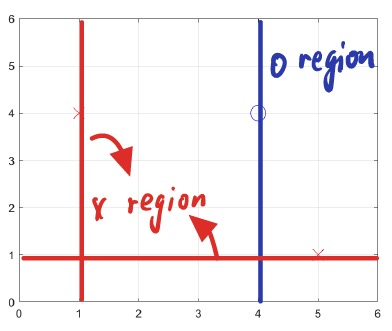
\includegraphics[width=0.4\textwidth]{images/1_NN.png}
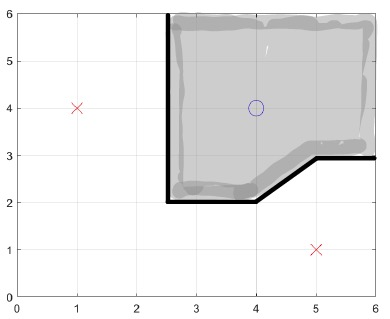
\includegraphics[width=0.4\textwidth]{images/2_NN.png} \\
c) $L_2$ \qquad \qquad \qquad \qquad \qquad \qquad \qquad \qquad d) $L_{\inf}$\\
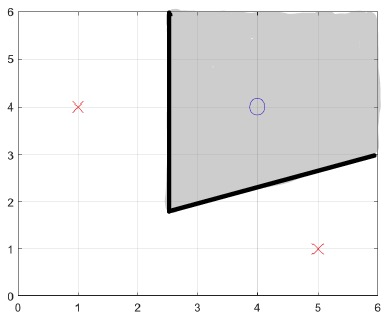
\includegraphics[width=0.4\textwidth]{images/3_NN.png}
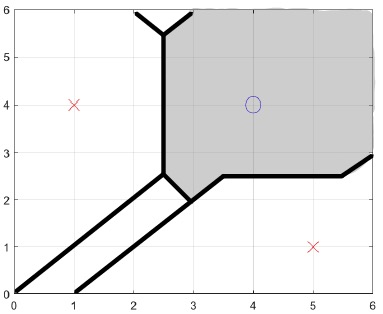
\includegraphics[width=0.4\textwidth]{images/4_NN.png} \\

\end{enumerate}

